\documentclass{ctexart}

\usepackage{amsmath}

\usepackage{amsthm}

\usepackage{amssymb}

\usepackage{bm}

\usepackage{graphicx}

\usepackage{listings}
\lstset{
basicstyle=\scriptsize
}

\usepackage{caption}

\begin{titlepage}

\title{微分方程数值解 \\ 第五周作业}

\author{于慧倩 \\ 14300180118}

\date{2017年3月}

\end{titlepage}

\begin{document}

\maketitle

\newpage

\begin{enumerate}
%第一题
\item
给出修正和改进Euler格式的稳定性分析和绝对稳定区间。

对于改进的Euler格式,由\(u_{n+1}=u_n+ \frac{\Delta t}{2}(f_n+f_{n+1})\)可以得到
\[ u_n=(\frac{2+\Delta t a }{2-\Delta t a})^n u_0\]

 所以对于舍入误差有
 \[ |u_n^\epsilon -u_n|=(\frac{2+\Delta t a }{2-\Delta t a})^n \epsilon \]
 
 稳定性即希望初始的的舍入误差对固定的\(\delta t\),当\(n \rightarrow \infty\)时,仍然可以控制,即必须有\( |\frac{2+\Delta ta }{2- \Delta ta}| \leq 1 \)
 
 
令变量\(z=a \Delta t\),则对于改进的Euler格式,\(z\)必须落在\(|\frac{2+z }{2-z}| \leq 1\),并且\(z\) 可以是复的。由\(z=x+yi\)解出\(x \leq 0\)。
 即\(z\)必须落在左半平面内,如下图所示:
 
 \centerline{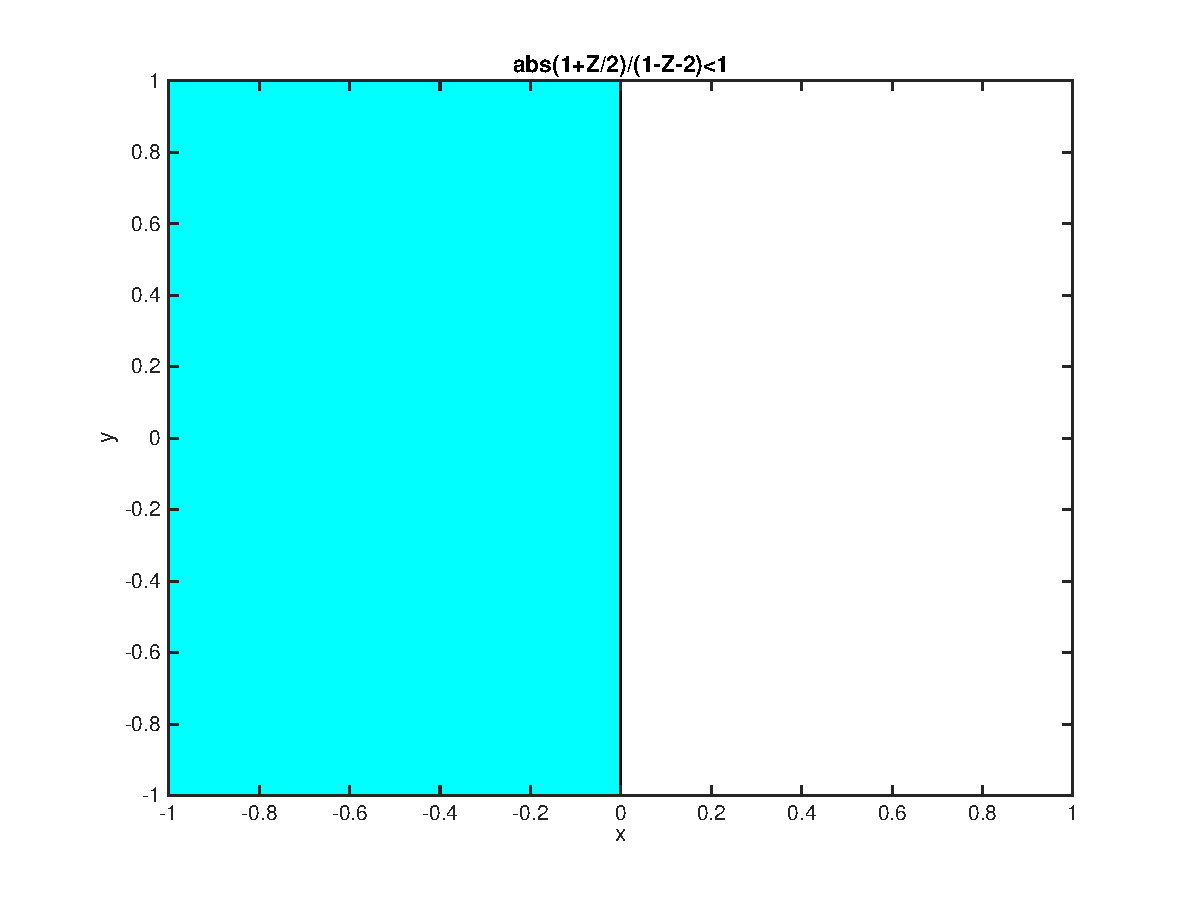
\includegraphics[width=5.5in]{5.eps}}
 
 同理对于修正的Euler格式,\( u_{n+1}=u_n+\Delta t a(u_n+ \frac{\Delta t}{2}au_n)\),可以得到\(u_n=(1+a\Delta t +\frac{1}{2}a^2\Delta t^2)u_n\)。继而有
 \[ u_n=(1+a\Delta t +\frac{1}{2}a^2\Delta t^2)^nu_0\]
 因此对于舍入误差有
 \[ |u_n^\epsilon -u_n| =(1+a\Delta t +\frac{1}{2}a^2\Delta t^2)^n \epsilon\]
 我们要求\(|1+a\Delta t +\frac{1}{2}a^2\Delta t^2| \leq 1\),令变量\(z=a \Delta t\),对于修正的Euler格式,\(|1+z +\frac{1}{2}z^2| \leq 1\),如下图所示:
 
 \centerline{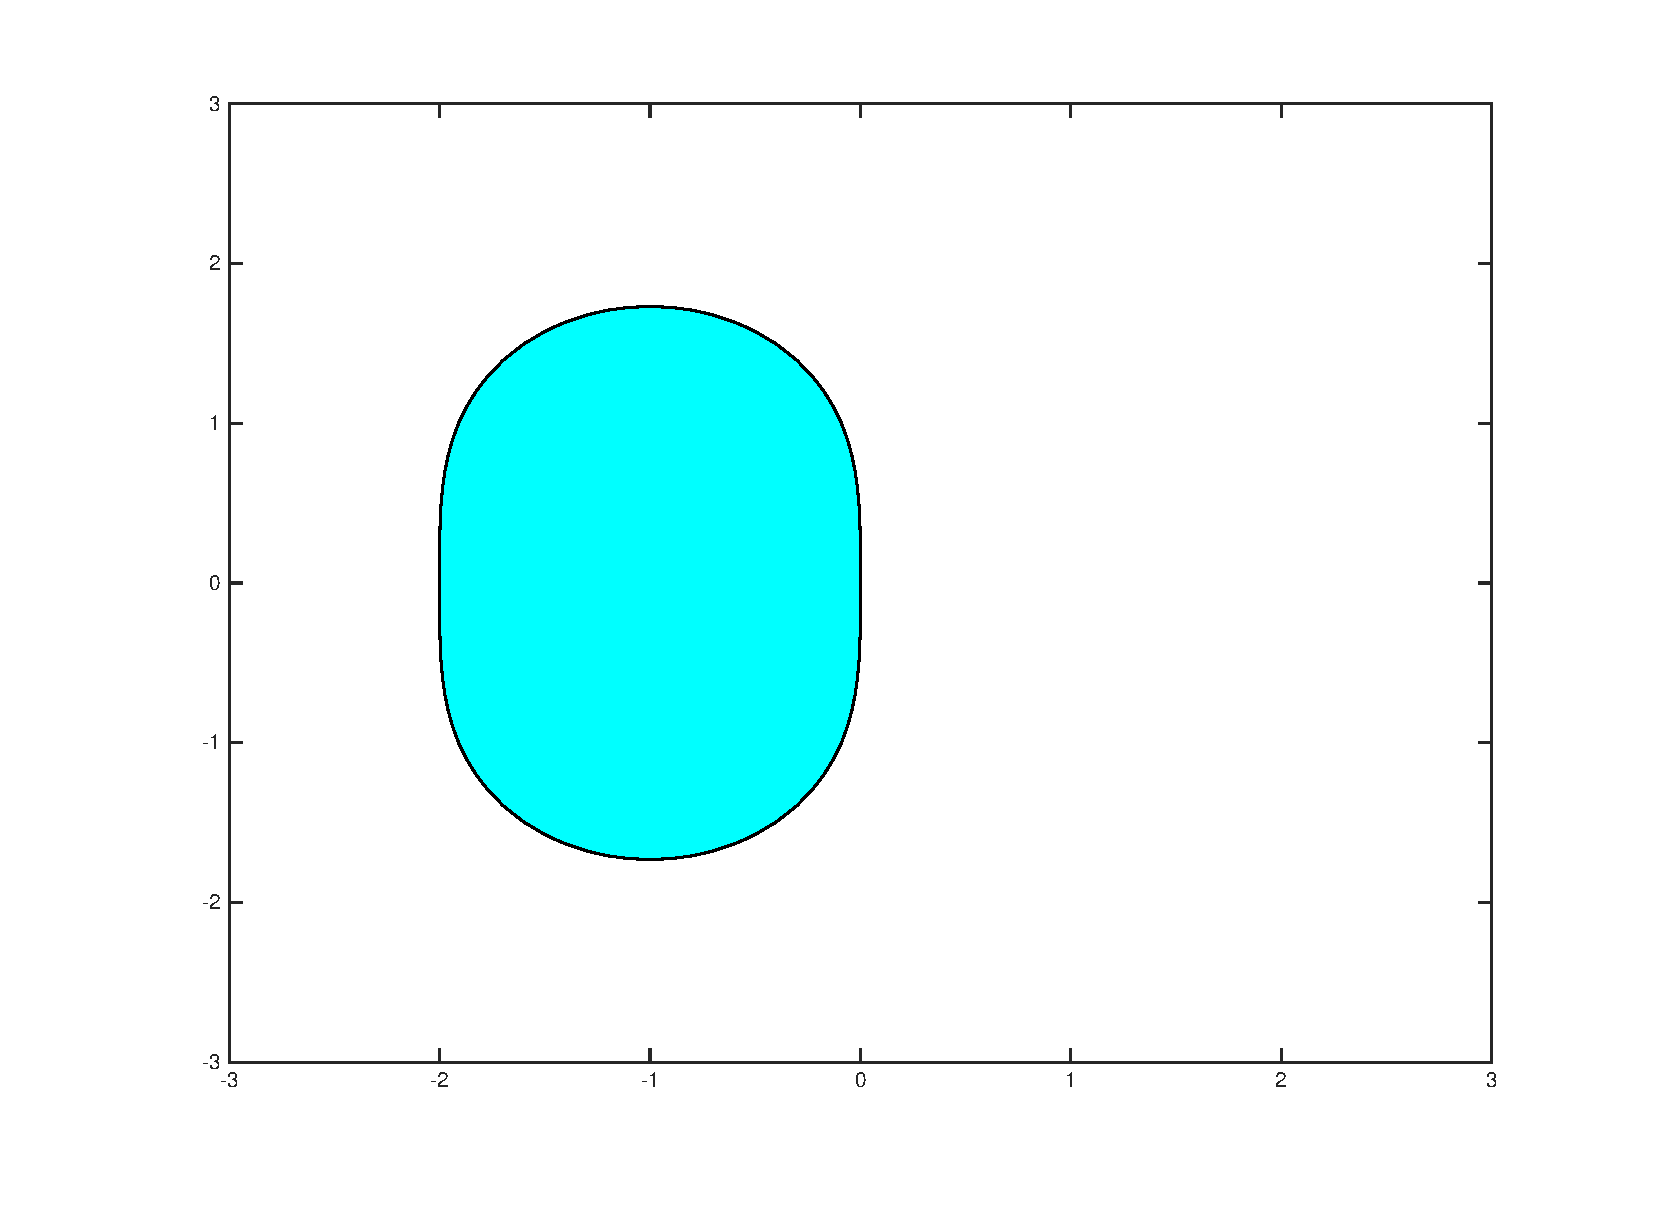
\includegraphics[width=5.5in]{4.eps}}

\item
用Taylor级数法(q=2,3)与Euler显式格式比较计算:
\[ \frac{\mbox{d} u}{\mbox{d}t} = u-u^2\]

Euler显式格式、Taylor级数(q=2,3)依次为下图:

\centerline{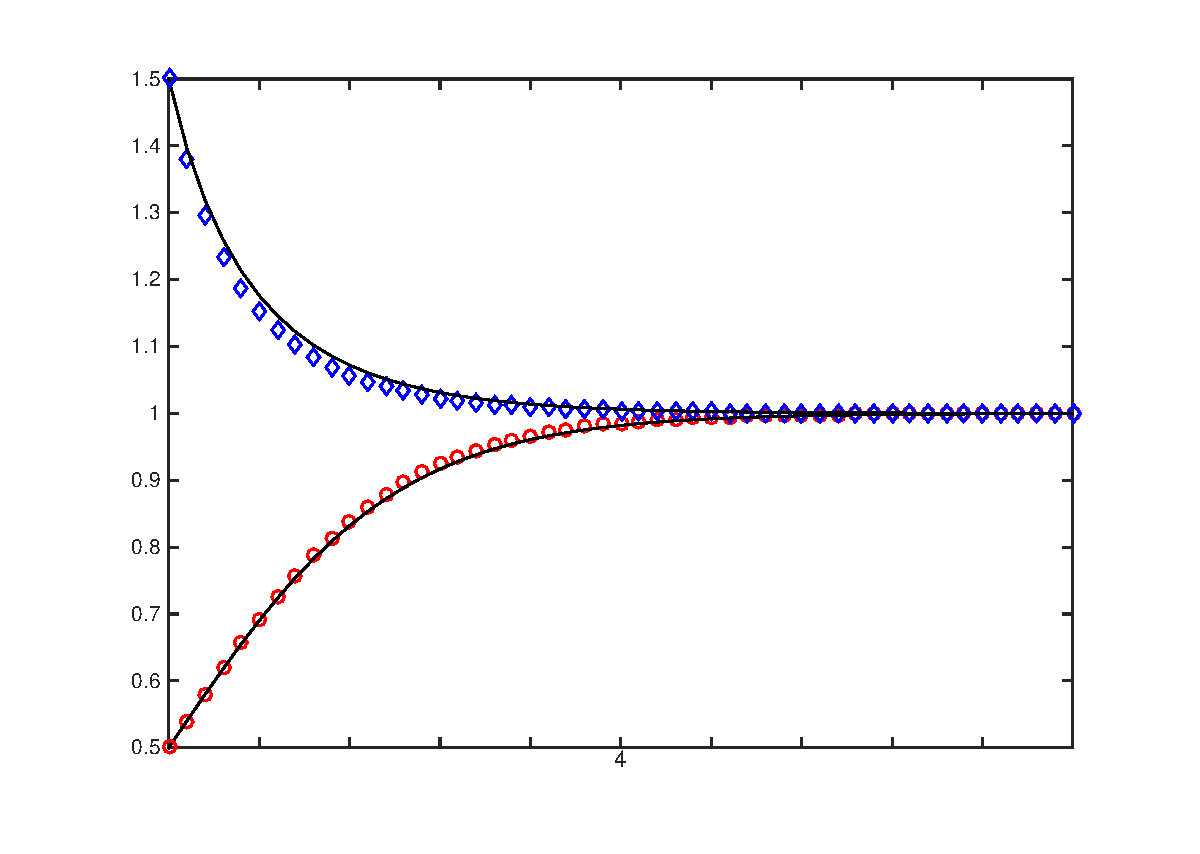
\includegraphics[width=3in]{1.eps}}
\centerline{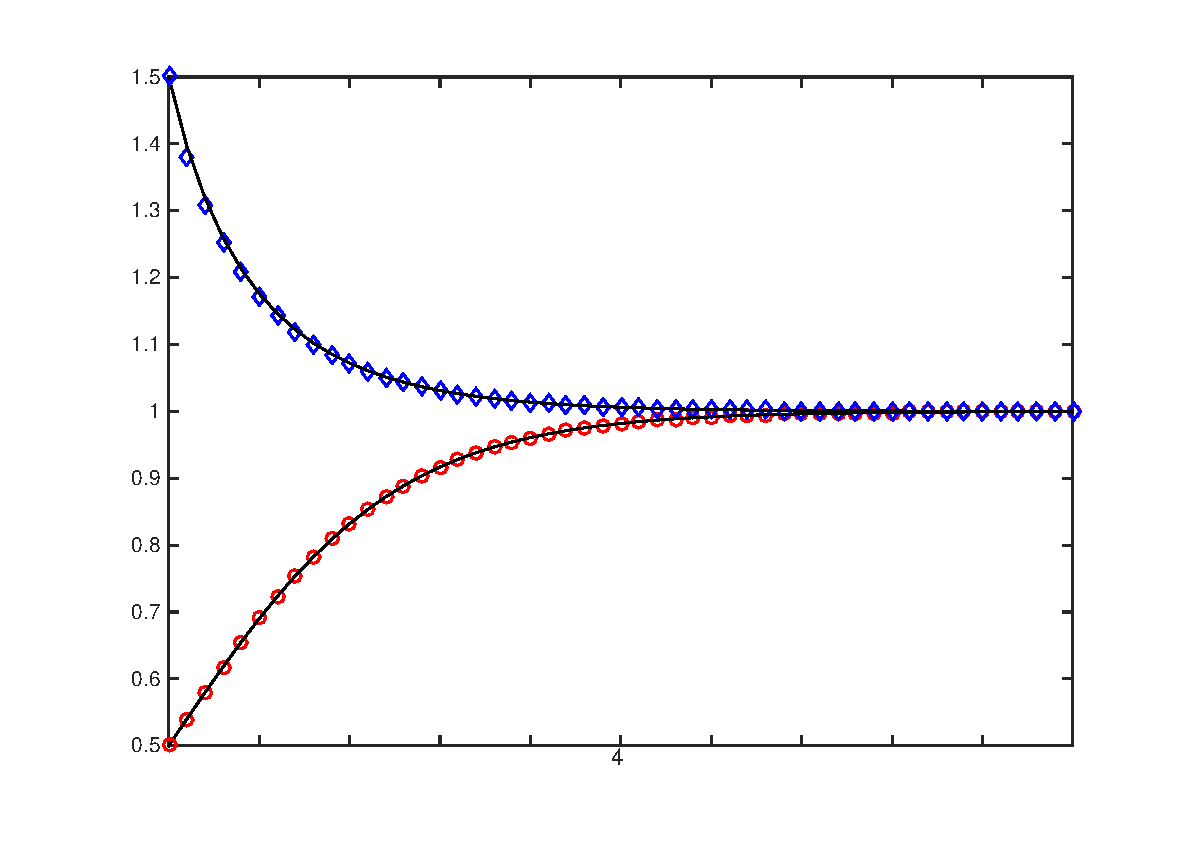
\includegraphics[width=3in]{2.eps}}
\centerline{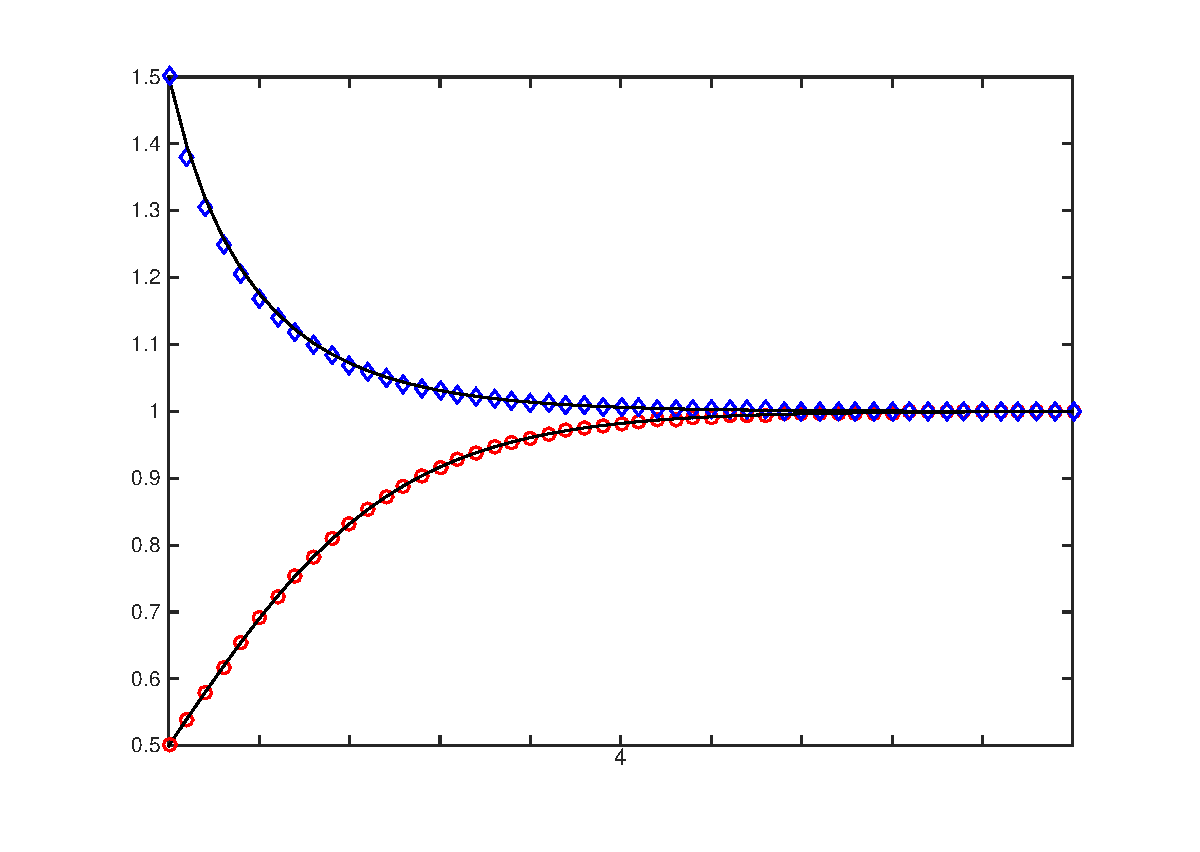
\includegraphics[width=3in]{3.eps}}
   
 进一步可以画出\(O(\Delta t^\rho) \sim \|u_T-u_N\|\)图像,如下:
 
 \centerline{\includegraphics[width=5.5in]{1总.eps}}
 可见q=3的Taylor级数法收敛最快。而对于q=3的Taylor级数法\(\Delta t< 2^{-13}\)时,减少步长不能再改进精度,因为此时误差已经接近机器精度。
 
 \item
 用二到四阶格式计算例2.2.2,观察收敛阶。
 
用步长\(\Delta t =2^{-i}\)作为步长,并与Euler显式(一阶)格式比较计算得到下图:

\centerline{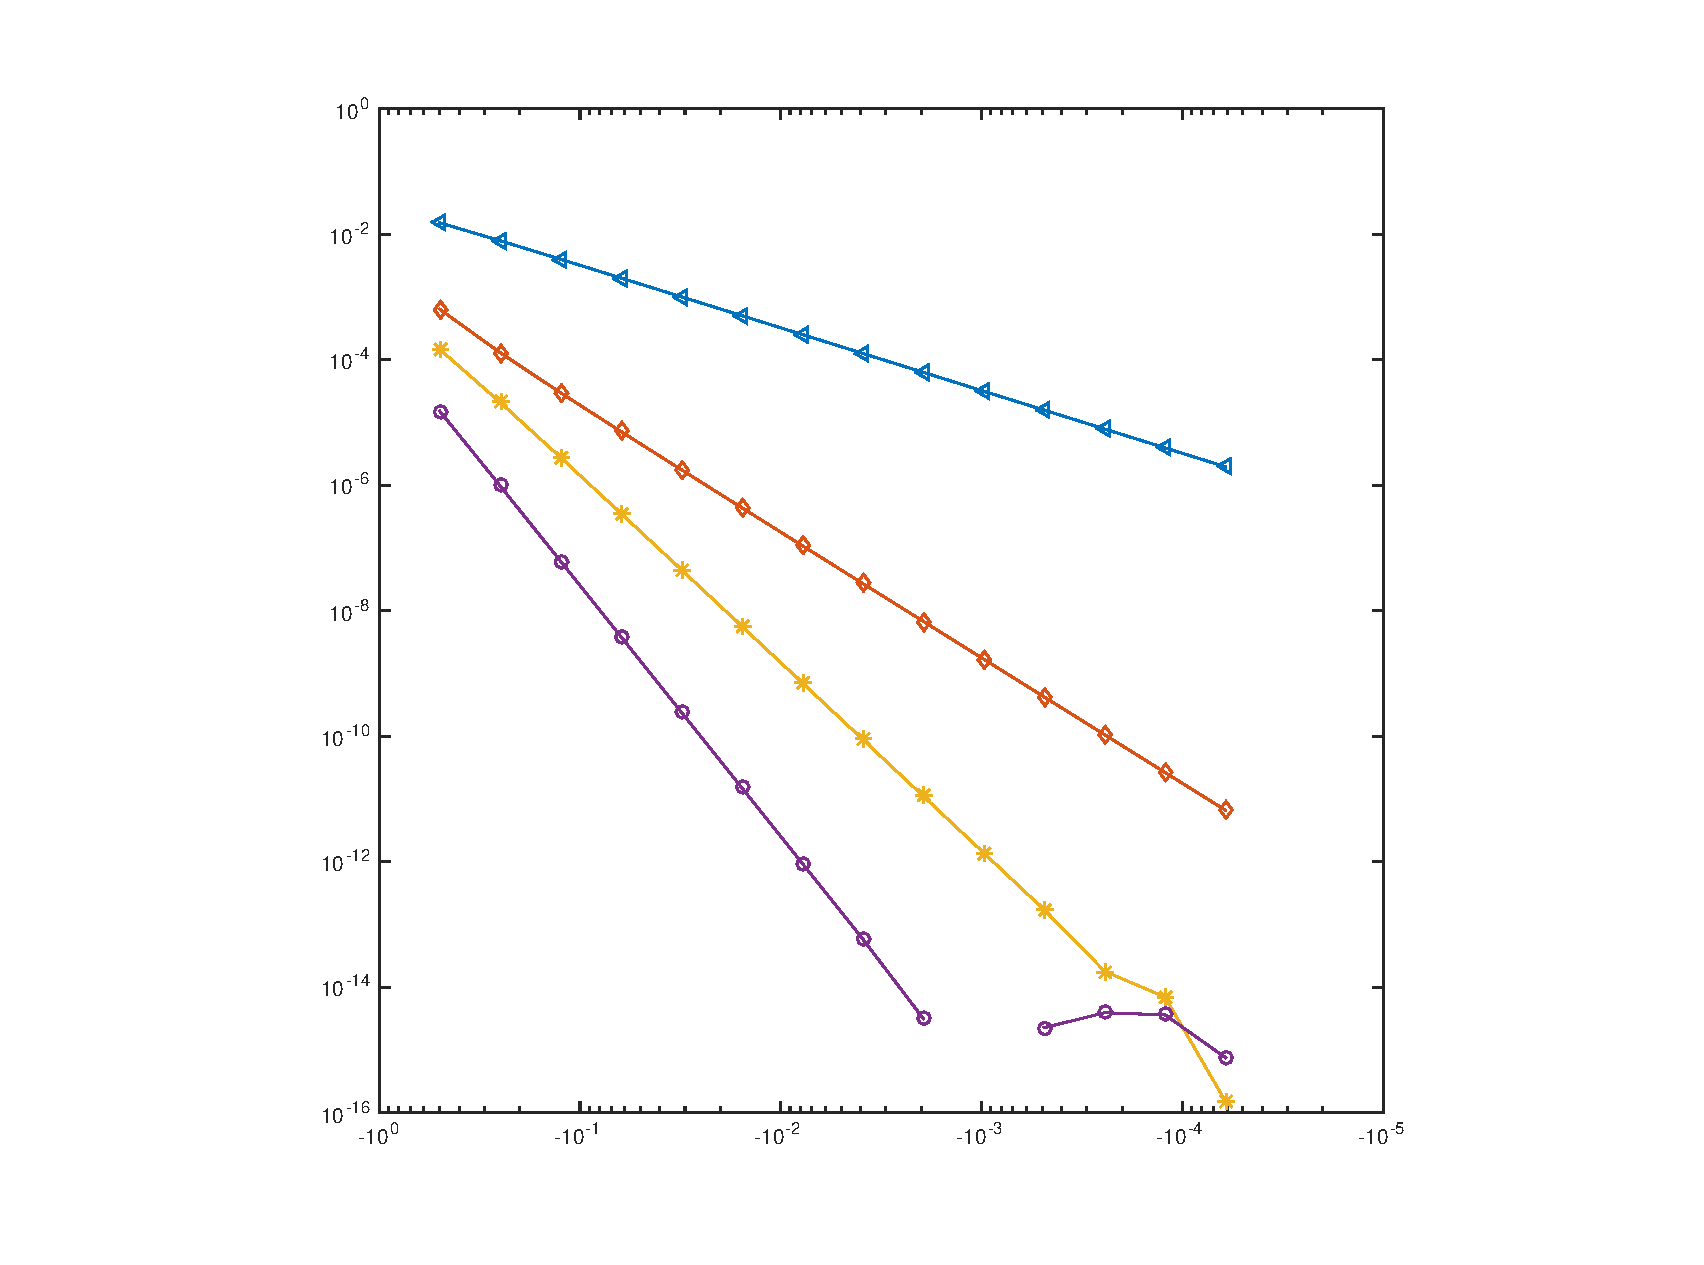
\includegraphics[width=5.5in]{last.eps}}

由于\(\ln |e_N|= \ln C -p I \ln 2\),所画(loglog)图像的斜率的绝对值代表了收敛阶,从图上可以估计出误差曲线所代表的收敛格式。同时对于高阶收敛,当\(\Delta t< 2^{-13}\)时,减少步长不能再改进精度,因为此时误差已经接近机器精度。






\end{enumerate}
\end{document}



